\section[Possible solutions]{Possible solutions}


\begin{frame}{Ethereum smart contracts}

\emph{figure to add}
\emph{citation to add }
%https://ieeexplore.ieee.org/document/8406325

\begin{itemize}
\item Based on the Ethereum blockchain
\item Each certification authority (CA) has \mg{smart contracts} that store a list of issued certificates and a revocation list
\item Specific format for certificates: \mg{hybrid certificates}
%\vspace{2mm}
\item Pros:
\begin{itemize}
\item Scalability: No size limit, no need to scroll the whole blockchain
\end{itemize}
\item Cons:
\begin{itemize}
\item Hard to use and to modify, not generic
\item Hybrid certificates
\item Transaction fees
\end{itemize}

\end{itemize}

%\begin{center}
%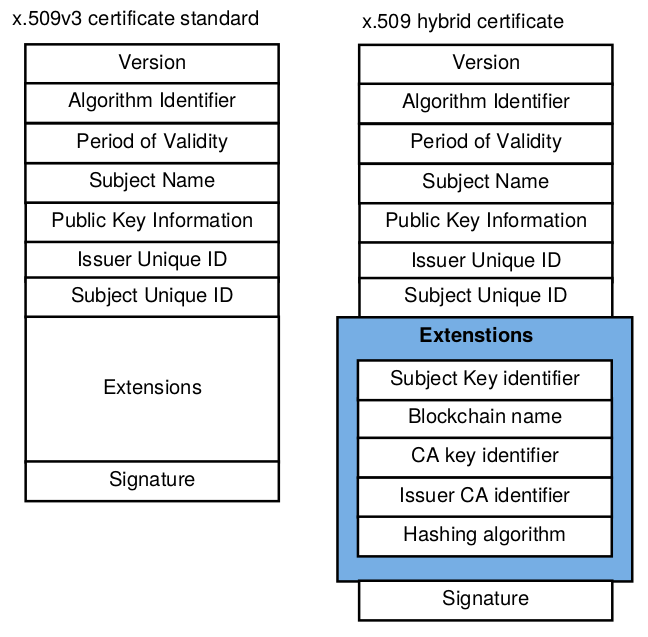
\includegraphics{figs/article_pki_blockchain.png}
%\end{center}

\end{frame}





\begin{frame}{Data fields in Bitcoin-based blockchains}

\begin{itemize}
\item \mg{OP\_RETURN} field that can contain data
\item Several blockchains could be used, such as Bitcoin or Namecoin
%\vspace{2mm}
\item Pros:
\begin{itemize}
\item Easy to implement, no hard fork required
\end{itemize}
\item Cons:
\begin{itemize}
\item No permissions: anyone can mine
\item Bitcoin: small size of the field (80 bytes), only fingerprints of certificates
\item Transaction fees
\item No easy revocation protocol
\item Burns bitcoins: they might not be used afterwards
\item The whole blockchain has to be read each time
\end{itemize}

\end{itemize}

\end{frame}





\begin{frame}{New blockchain}
\emph{here we describe the main points of our solution}

\begin{itemize}
\item Creation of a new blockchain with the \mg{Multichain} tool
\item Pros:
\begin{itemize}
\item Very customizable
\item Free transactions
\item Data of any length
\item Permission management
\end{itemize}
\item Cons:
\begin{itemize}
\item None :)
\end{itemize}


\end{itemize}
\end{frame}


